\paragraph{QuizziPedia::Front-End::Views::OtherUserView}

\label{QuizziPedia::Front-End::View::OtherUserViewtView}
\begin{figure} [ht]
	\centering
	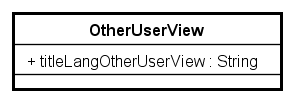
\includegraphics[scale=0.80]{UML/Classi/Front-End/QuizziPedia_Front-end_Views_OtherUserView.png}
	\caption{QuizziPedia::Front-End::Views::OtherUserView}
\end{figure} \FloatBarrier
\begin{itemize}
	\item \textbf{Descrizione}: \textit{view\ped{G}} contenente le direttive dei dati personali e delle statistiche di un utente ricercato;
	\item \textbf{Utilizzo}: viene visualizzata dopo la ricerca e permette all'utente che ha l'ha effettuata di visualizzare i dati personali e le statistiche di un utente ricercato;
	\item \textbf{Relazioni con altre classi}:
	\begin{itemize}
		\item \textbf{IN \texttt{StatisticsDirective}}: directive che permette di visualizzare le statistiche di un utente;
		\item \textbf{IN \texttt{UserDetailsDirective}}: directive che permette di visualizzare i dati personali di un utente;
		\item \textbf{IN \texttt{LangModel}}: rappresenta il modello delle informazioni per la giusta traduzione dell'applicazione.
	\end{itemize}
	\item \textbf{Attributi}:
	\begin{itemize}
		\item \texttt{+ titleLangOtherUserView: String} \\ Attributo che viene utilizzato per visualizzare la giusta traduzione del titolo della pagina, in italiano o in inglese.
	\end{itemize}
\end{itemize}